\documentclass[journal,12pt,twocolumn]{IEEEtran}

\usepackage{setspace}
\usepackage{gensymb}
\singlespacing
\usepackage[cmex10]{amsmath}

\usepackage{amsthm}

\usepackage{mathrsfs}
\usepackage{txfonts}
\usepackage{stfloats}
\usepackage{bm}
\usepackage{cite}
\usepackage{cases}
\usepackage{subfig}

\usepackage{longtable}
\usepackage{multirow}

\usepackage{enumitem}
\usepackage{mathtools}
\usepackage{steinmetz}
\usepackage{tikz}
\usepackage{circuitikz}
\usepackage{verbatim}
\usepackage{tfrupee}
\usepackage[breaklinks=true]{hyperref}
\usepackage{graphicx}
\usepackage{tkz-euclide}

\usetikzlibrary{calc,math}
\usepackage{listings}
    \usepackage{color}                                            %%
    \usepackage{array}                                            %%
    \usepackage{longtable}                                        %%
    \usepackage{calc}                                             %%
    \usepackage{multirow}                                         %%
    \usepackage{hhline}                                           %%
    \usepackage{ifthen}                                           %%
    \usepackage{lscape}     
\usepackage{multicol}
\usepackage{chngcntr}

\DeclareMathOperator*{\Res}{Res}

\renewcommand\thesection{\arabic{section}}
\renewcommand\thesubsection{\thesection.\arabic{subsection}}
\renewcommand\thesubsubsection{\thesubsection.\arabic{subsubsection}}

\renewcommand\thesectiondis{\arabic{section}}
\renewcommand\thesubsectiondis{\thesectiondis.\arabic{subsection}}
\renewcommand\thesubsubsectiondis{\thesubsectiondis.\arabic{subsubsection}}


\hyphenation{op-tical net-works semi-conduc-tor}
\def\inputGnumericTable{}                                 %%

\lstset{
%language=C,
frame=single, 
breaklines=true,
columns=fullflexible
}
\begin{document}

\newcommand{\BEQA}{\begin{eqnarray}}
        \newcommand{\EEQA}{\end{eqnarray}}
\newcommand{\define}{\stackrel{\triangle}{=}}
\bibliographystyle{IEEEtran}
\raggedbottom
\setlength{\parindent}{0pt}
\providecommand{\mbf}{\mathbf}
\providecommand{\pr}[1]{\ensuremath{\Pr\left(#1\right)}}
\providecommand{\qfunc}[1]{\ensuremath{Q\left(#1\right)}}
\providecommand{\sbrak}[1]{\ensuremath{{}\left[#1\right]}}
\providecommand{\lsbrak}[1]{\ensuremath{{}\left[#1\right.}}
\providecommand{\rsbrak}[1]{\ensuremath{{}\left.#1\right]}}
\providecommand{\brak}[1]{\ensuremath{\left(#1\right)}}
\providecommand{\lbrak}[1]{\ensuremath{\left(#1\right.}}
\providecommand{\rbrak}[1]{\ensuremath{\left.#1\right)}}
\providecommand{\cbrak}[1]{\ensuremath{\left\{#1\right\}}}
\providecommand{\lcbrak}[1]{\ensuremath{\left\{#1\right.}}
\providecommand{\rcbrak}[1]{\ensuremath{\left.#1\right\}}}
\theoremstyle{remark}
\newtheorem{rem}{Remark}
\newcommand{\sgn}{\mathop{\mathrm{sgn}}}
\providecommand{\abs}[1]{\vert#1\vert}
\providecommand{\res}[1]{\Res\displaylimits_{#1}}
\providecommand{\norm}[1]{\lVert#1\rVert}
%\providecommand{\norm}[1]{\lVert#1\rVert}
\providecommand{\mtx}[1]{\mathbf{#1}}
\providecommand{\mean}[1]{E[#1]}
\providecommand{\fourier}{\overset{\mathcal{F}}{ \rightleftharpoons}}
%\providecommand{\hilbert}{\overset{\mathcal{H}}{ \rightleftharpoons}}
\providecommand{\system}{\overset{\mathcal{H}}{ \longleftrightarrow}}
%\newcommand{\solution}[2]{\textbf{Solution:}{#1}}
\newcommand{\solution}{\noindent \textbf{Solution: }}
\newcommand{\cosec}{\,\text{cosec}\,}
\newcommand{\comb}[2]{{}^{#1}\mathrm{C}_{#2}}
\providecommand{\dec}[2]{\ensuremath{\overset{#1}{\underset{#2}{\gtrless}}}}
\newcommand{\myvec}[1]{\ensuremath{\begin{pmatrix}#1\end{pmatrix}}}
\newcommand{\mydet}[1]{\ensuremath{\begin{vmatrix}#1\end{vmatrix}}}
\numberwithin{equation}{subsection}
\makeatletter
\@addtoreset{figure}{problem}
\makeatother
\let\StandardTheFigure\thefigure
\let\vec\mathbf
\renewcommand{\thefigure}{\theproblem}
\def\putbox#1#2#3{\makebox[0in][l]{\makebox[#1][l]{}\raisebox{\baselineskip}[0in][0in]{\raisebox{#2}[0in][0in]{#3}}}}
\def\rightbox#1{\makebox[0in][r]{#1}}
\def\centbox#1{\makebox[0in]{#1}}
\def\topbox#1{\raisebox{-\baselineskip}[0in][0in]{#1}}
\def\midbox#1{\raisebox{-0.5\baselineskip}[0in][0in]{#1}}
\vspace{3cm}
\title{AI1103 Assignment-2}
\author{SRIVATSAN T - CS20BTECH11062}
\maketitle
\newpage
\bigskip
\renewcommand{\thefigure}{\theenumi}
\renewcommand{\thetable}{\theenumi}
Download all python codes from
\begin{lstlisting}
https://github.com/CS20BTECH11062/AI1103/tree/main/Assignment-2/codes
\end{lstlisting}
%
and latex-tikz codes from
%
\begin{lstlisting}
https://github.com/CS20BTECH11062/AI1103/tree/main/Assignment-2/Assignment-2.tex
\end{lstlisting}
\section*{QUESTION (GATE Prob 27)}
A fair coin is tossed 10 times. What is the \\probability that ONLY the first 2 tosses will yield heads?
\section*{SOLUTION}
Let M be a random variable representing number of 'heads' in 10 tosses.\\
So M has a binomial distribution :
\begin{align}
    \pr{M=k} = \comb{n}{k} \times (h)^{n-k} \times (t)^{k}\label{0.0.1}
\end{align}
Where
\begin{itemize}
    \item n = Total number of tosses = 10
    \item h = Probability that 'head' appears in a toss = \( \frac{1}{2} \)
    \item t = Probability that 'tail' appears in a toss = \( \frac{1}{2} \)
\end{itemize}
\bigskip
So,
\begin{align}
    \pr{M=k} = \comb{10}{k} \times \brak{\frac{1}{2}}^{10-k} \times \brak{\frac{1}{2}}^{k}\label{0.0.2}
\end{align}
\begin{table}[h]
    \begin{center}
        \resizebox{7cm}{!}
        {
            \begin{tabular}{|c|c|}
                \hline
                n           & 10                                                                            \\
                \hline
                $\pr{2 heads}$  & $\pr{X = 2}$                                                                    \\
                \hline
                Calculation & $\comb{10}{2} \times \brak{\frac{1}{2}}^{10-2} \times \brak{\frac{1}{2}}^{2}$ \\
                \hline
                Value       & 0.043945                                                                      \\
                \hline
            \end{tabular}
        }
    \end{center}
\end{table}
\begin{itemize}
    \item Now, these 2 heads can occur at any position in 10 tosses.
    \item Number of ways of choosing 2 positions from 10 tosses = $\comb{10}{2}$
          \bigskip
    \item Probability that chosen 2 'heads' are from FIRST and SECOND tosses = \(\displaystyle \frac{1}{\comb{10}{2}}\)
          \bigskip
\end{itemize}
Probability that ONLY the first 2 tosses yield heads =  $\pr{M = 2} \times$ Probability that chosen 2 'heads' are from FIRST and SECOND tosses.
\bigskip
\begin{align}
    \implies \comb{10}{2} \times \brak{\frac{1}{2}}^{10} \times \frac{1}{\comb{10}{2}} = \brak{\frac{1}{2}}^{10}\notag
\end{align}
Probability that 'head' appears ONLY in the first two tosses is $\displaystyle\brak{\frac{1}{2}}^{10}$\\
\begin{center}
    Correct Option : C
\end{center}
\pagebreak
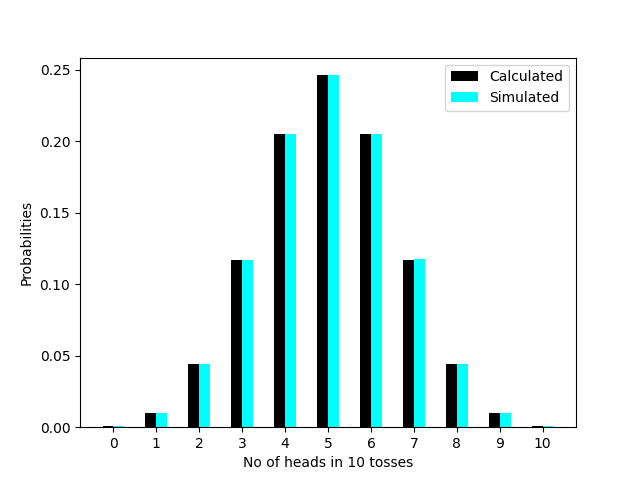
\includegraphics{Figure-1.png}
\end{document}